\chapter{Sorting Algorithms}

\section{Counting Sort $o(n)$}
\textbf{{\Large{Problem Description}}}

Given an (unsorted) array of n elements, can we sort them in $O(n)$ time?\newline
    
\textbf{{\Large{Solution}}}\newline\newline
\textbf{{\large{Sorting in Linear Time (Counting Sort)}}}\newline\newline
If the array A contains n integers with small range \textbf{[L..R]}, we can use the Counting Sort algorithm. For the explanation
below, assume that array A is \textbf{{2, 5, 2, 2, 3, 3}}. The idea of Counting Sort is as follows:

1. Prepare a \textbf{‘frequency array’ f} with size $k$ = $R-L+1$ and initialize f with zeroes.
On the example array above, we have $L$ = 2, $R$ = 5, and k = 4.
\newline
\\
2. We do one pass through array A and update the frequency of each integer that we see,
i.e. for each i ∈ [0..n-1], we do \textbf{f[A[i]-L]++}.
On the example array above, we have \textbf{f[0] = 3, f[1] = 2, f[2] = 0, f[3] = 1}.
\newline
\\
3. Once we know the frequency of each integers in that small range,
we compute the prefix sums of each i, i.e. \textbf{f[i] = [f-1] + f[i] ∀i ∈ [1..k-1]}.
Now, f[i] contains the number of elements less than or equal to i.
On the example array above, we have \textbf{f[0] = 3, f[1] = 5, f[2] = 5, f[3] = 6.}
\newline
\\
4. Next, go backwards from i = n-1 down to i = 0.
We place \textbf{A[i]} at index f[A[i]-L]-1 as it is the correct location for \textbf{A[i]}. We decrement \textbf{f[A[i]-L]} by one so that the next copy of \textbf{A[i]}—if any—will be placed right before the current \textbf{A[i]}. On the example array above, we first put A[5] = 3 in index \textbf{f[A[5]-2]-1 = f[1]-1 = 5-1 = 4} and decrement \textbf{f[1] to 4}. Next, we put \textbf{A[4] = 3}—the same value as \textbf{A[5] = 3}—now in index \textbf{f[A[4]-2]-1 = f[1]-1 = 4-1 = 3} and decrement f[1] to 3. Then, we put \textbf{A[3] = 2} in index \textbf{[A[3]-2]-1 = 2} and decrement \textbf{f[0] to 2}. We repeat the next three steps until we obtain a sorted array: \textbf{{2, 2, 2, 3, 3, 5}}. The time complexity of Counting Sort is $O(n+k)$.
\newline
\\
\textbf{{\Large{Implementation}}}

\begin{lstlisting}{c++}
        #include <bits/stdc++.h>
        
        using namespace std;
        int noOfElements;
        
        void countingSort(vector<int> &v){
            int max_ele = *max_element(v.begin(), v.end());
            vector<int> count_(max_ele + 1, 0);
            for(int i = 0; i < (int)v.size(); ++i)count_[ v[i] ]++;
            for(int i = 1; i <= max_ele; ++i)count_[ i ] += count_[ i - 1 ];
        
            vector<int> new_array( (int)v.size() );
            for(int i = 0; i < (int)v.size(
                                           ); ++i){
                new_array[ count_[ v[i] ]  - 1 ] = v[i];
                count_[ v[i] ]--;
            }
            for(int i = 0; i < (int)v.size(); ++i){
                cout << new_array[i] << " ";
            }
        
        }
        int main(){
            cin >> noOfElements;
            vector<int> v(noOfElements);
            for(int i = 0; i < noOfElements; ++i)cin >> v[i];
            countingSort(v);
        }
\end{lstlisting}

\newpage

\section{Bubble Sort $o(n^2)$} 
\textbf{{\Large{Description}}}

Bubble Sort is the simplest sorting algorithm that works by repeatedly swapping the adjacent elements if they are in wrong order.\newline
    
\textbf{{\Large{Solution}}}\newline\newline
\textbf{{\large{Example:}}}\newline\footnotetext{\url{https://www.geeksforgeeks.org/bubble-sort/}}

1. \textbf{First Pass:}\newline
( \textbf{5 1} 4 2 8 ) –$>$ ( \textbf{1 5} 4 2 8 ), Here, algorithm compares the first two elements, and swaps since 5 $>$ 1.\newline
( 1 \textbf{5 4} 2 8 ) –$>$  ( 1 \textbf{4 5} 2 8 ), Swap since 5 $>$ 4\newline
( 1 4 \textbf{5 2} 8 ) –$>$  ( 1 4\textbf{ 2 5} 8 ), Swap since 5 $>$ 2\newline
( 1 4 2 \textbf{5 8} ) –$>$ ( 1 4 2 \textbf{5 8} ), Now, since these elements are already in order (8 $>$ 5), algorithm does not swap them.
\newline
\\
2. \textbf{Second Pass:}\newline
( \textbf{1 4} 2 5 8 ) –$>$ ( \textbf{1 4} 2 5 8 )\newline
( 1 \textbf{4 2} 5 8 ) –$>$ ( 1 \textbf{2 4} 5 8 ), Swap since 4 $>$ 2\newline
( 1 2 \textbf{4 5} 8 ) –$>$ ( 1 2 \textbf{4 5} 8 )\newline
( 1 2 4 \textbf{5 8} ) –$>$  ( 1 2 4 \textbf{5 8} )\newline
Now, the array is already sorted, but our algorithm does not know if it is completed. The algorithm needs one whole pass without any swap to know it is sorted.
\newline
\\
3. \textbf{Finally}\newline
( \textbf{1 2} 4 5 8 ) –$>$ ( \textbf{1 2} 4 5 8 )\newline
( 1 \textbf{2 4} 5 8 ) –$>$ ( 1 \textbf{2 4} 5 8 )\newline
( 1 2 \textbf{4 5} 8 ) –$>$ ( 1 2 \textbf{4 5} 8 )\newline
( 1 2 4 \textbf{5 8} ) –$>$ ( 1 2 4 \textbf{5 8} )\newline

\newline
\\
\newpage
\textbf{{\Large{Implementation}}}

\begin{lstlisting}{c++}
        #include <bits/stdc++.h>
        
        using namespace std;
        
        int n;
        void bubbleSort(vector<int> &arr){
        	for (int i = 0; i < n-1; ++i)
                for (int j = 0; j < n-i-1; j++)
                    if (arr[j] > arr[j+1])
                        swap(arr[j], arr[j+1]);
        
        }
        
        int main() {
            
        	cin >> n;
        	vector<int> arr(n);
        	for (int i = 0; i < n; ++i)cin >> arr[i];
        	bubbleSort(arr);
        	cout<<"Sorted array: \n";
        	///Print the array after sorting
        	for (int i = 0; i < n; ++i)cout << arr[i] << " ";
        	return 0;
        }
\end{lstlisting}
\newline\newline\newline
\\
\\
\textbf{{\Large{Optimized Implementation:}}}\newline\newline\
The above function always runs $O(n^2)$ time even if the array is sorted. It can be optimized by stopping the algorithm if inner loop didn’t cause any swap.
\newline
\begin{lstlisting}{c++}
        #include <bits/stdc++.h>
        
        using namespace std;
        
        int n;
        void bubbleSort(vector<int> &arr){
           bool swapped;
           for (int i = 0; i < n-1; i++) {
             swapped = false;
             for (int j = 0; j < n-i-1; j++){
                if (arr[j] > arr[j+1]) {
                   swap(arr[j], arr[j+1]);
                   swapped = true;
                }
             }
             // If no two elements were swapped by inner loop, then break.
             if (swapped == false)
                break;
           }
        }
        
        int main() {
        
        	cin >> n;
        	vector<int> arr(n);
        	for (int i = 0; i < n; ++i)cin >> arr[i];
        	bubbleSort(arr);
        	cout<<"Sorted array: \n";
        	///Print the array after sorting
        	for (int i = 0; i < n; ++i)cout << arr[i] << " ";
        	return 0;
        }
\end{lstlisting}


\newpage


\section{Insertion Sort $o(n^2)$}
\textbf{{\Large{Description}}}

Insertion sort is a simple sorting algorithm that works the way we sort playing cards in our hands.
.\newline
    
\textbf{{\Large{Solution}}}\newline\newline
\textbf{{\large{Consider This Figuer:}}}\newline\footnotetext{\url{https://www.geeksforgeeks.org/selection-sort/}}
\begin{figure}[h]
    \centering
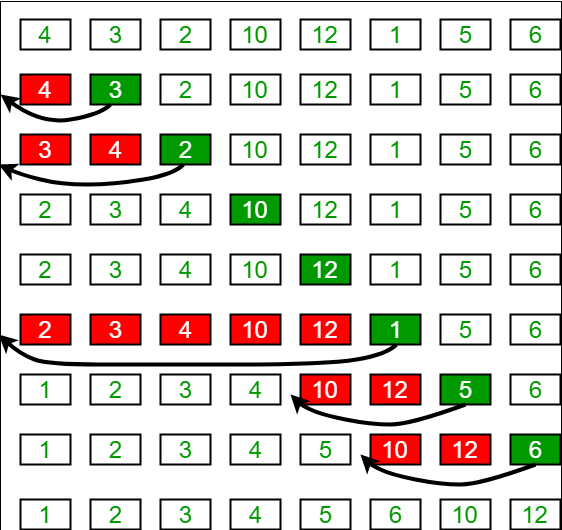
\includegraphics[width=10cm, height=6cm]{insertion-sort.png}
 \caption{Insertion Sort Execution Example}\footnotemark
    \label{fig:insertion-sort}
\end{figure}
\footnotetext{\url{https://media.geeksforgeeks.org/wp-content/uploads/insertionsort.png}}
\newline
\\
\newpage
\textbf{{\Large{Implementation}}}

\begin{lstlisting}{c++}
        #include <bits/stdc++.h>
        
        using namespace std;
        
        int n;
        void insertionSort(vector<int> &arr){
        	int key, j;
        	for (int i = 1; i < n; i++) {
        		key = arr[i];
        		j = i - 1;
        		/* Move elements of arr[0..i-1], that are
        		greater than key, to one position ahead
        		of their current position */
        		while (j >= 0 && arr[j] > key)
        		{
        			arr[j + 1] = arr[j];
        			j = j - 1;
        		}
        		arr[j + 1] = key;
        	}
        }
        int main(){
            cin >> n;
        	vector<int> arr(n);
            for(int i = 0; i < n; ++i)cin >> arr[i];
        	insertionSort(arr);
        	cout << "Array after sorting: ";
        	for(int i = 0; i < n; ++i)cout << arr[i] << " ";
        
        	return 0;
        }

\end{lstlisting}
\newpage
\section{Selection Sort $o(n^2)$}

%klsdfj;lskdjf;klsdj;lsdj;lsdrkjg;lskrj;flksrj;glsrkj;glsrjkg;lr

The $selection sort algorithm$ sorts an array by repeatedly finding the $minimum$ element (considering ascending order) from $unsorted part$ and putting it at the beginning. The $algorithm$ maintains two $subarrays$ in a given array.\newline

1) The subarray which is already sorted.\newline
2) Remaining subarray which is unsorted.\newline

In every iteration of selection sort, the minimum element (considering ascending order) from the unsorted subarray is picked and moved to the sorted subarray.\newline
    
\textbf{{\Large{Example\footnotetext{\url{https://www.geeksforgeeks.org/selection-sort/}}}}}
\begin{lstlisting}{c++}
        arr[] = 64 25 12 22 11
        
        // Find the minimum element in arr[0...4]
        // and place it at beginning
        11 25 12 22 64
        
        // Find the minimum element in arr[1...4]
        // and place it at beginning of arr[1...4]
        11 12 25 22 64
        
        // Find the minimum element in arr[2...4]
        // and place it at beginning of arr[2...4]
        11 12 22 25 64
        
        // Find the minimum element in arr[3...4]
        // and place it at beginning of arr[3...4]
        11 12 22 25 64 

\end{lstlisting}
\\
\\
\newline\newline
\textbf{{\Large{Implementation}}}
\begin{lstlisting}{c++}
        #include <bits/stdc++.h>
        
        using namespace std;
        
        int n;
        void selectionSort(vector<int> &arr){
        	int min_idx;
        	// One by one move boundary of unsorted subarray
        	for (int i = 0; i < n-1; i++) {
        		// Find the minimum element in unsorted array
        		min_idx = i;
        		for (int j = i+1; j < n; j++)
        		if (arr[j] < arr[min_idx])
        			min_idx = j;
        
        		// Swap the found minimum element with the first element
        		swap(arr[min_idx], arr[i]);
        	}
        }
        
        int main(){
            cin >> n ;
        	vector<int> arr(n);
        	for (int i=0; i < n; i++)cin >> arr[i];
        	selectionSort(arr);
        	cout << "Sorted array: \n";
        	for (int i=0; i < n; i++)cout << arr[i] << " ";
        	return 0;
        }
\end{lstlisting}

\newpage





\section{Merge Sort $o(nlogn)$}\footnotetext{\url{https://www.hackerearth.com/practice/algorithms/sorting/merge-sort/tutorial/}}
Merge sort is a divide-and-conquer algorithm based on the idea of breaking down a list into several sub-lists until each sublist consists of a single element and merging those sublists in a manner that results into a sorted list.\newline

Idea:

1. Divide the unsorted list into $N$ sublists, each containing  $1$ element.

2. Take adjacent pairs of two singleton lists and merge them to form a list of $2$ elements. N will now convert into $N $/$ 2$ lists of size $2$.

3. Repeat the process till a single sorted list of obtained.

\hspace{7mm}While comparing two sublists for merging, the first element of both lists is taken into consideration. While sorting in ascending order, the element that is of a lesser value becomes a new element of the sorted list. This procedure is repeated until both the smaller sublists are empty and the new combined sublist comprises all the elements of both the sublists.

Now consider the following recursive function:
\begin{lstlisting}{c++}
        arr[] = 64 25 12 22 11
        
        // Find the minimum element in arr[0...4]
        // and place it at beginning
        11 25 12 22 64
        
        // Find the minimum element in arr[1...4]
        // and place it at beginning of arr[1...4]
        11 12 25 22 64
        
        // Find the minimum element in arr[2...4]
        // and place it at beginning of arr[2...4]
        11 12 22 25 64
        
        // Find the minimum element in arr[3...4]
        // and place it at beginning of arr[3...4]
        11 12 22 25 64 

\end{lstlisting}
\\
\\
\newline\newline
\textbf{{\Large{Implementation}}}
\begin{lstlisting}{c++}
        void merge_sort (int A[] , int start , int end ){
            if( start < end ) {
                   int mid = (start + end ) / 2 ;// defines the current array in 2 parts .
                   merge_sort (A, start , mid ) ;// sort the 1st part of array .
                   merge_sort (A,mid+1 , end ) ;// sort the 2nd part of array.
        
                 // merge the both parts by comparing elements of both the parts.
                  merge(A,start , mid , end );   
           }                    
        }
\end{lstlisting}

\newpage

\section{Quick Sort $o(n^2)$}\footnotetext{\url{https://www.w3schools.in/data-structures-tutorial/sorting-techniques/quick-sort-algorithm/}}

Quick sort is one of the most famous sorting algorithms based on divide and conquers strategy which results in an O(n log n) complexity. So, the algorithm starts by picking a single item which is called pivot and moving all smaller items before it, while all greater elements in the later portion of the list. This is the main quick sort operation named as a partition, recursively repeated on lesser and greater sublists until their size is one or zero - in which case the list is wholly sorted. Choosing an appropriate pivot, as an example, the central element is essential for avoiding the severely reduced performance of $o(n^2)$.
\\
\\
\newline\newline
\textbf{{\Large{Implementation}}}
\begin{lstlisting}{c++}
        #include <bits/stdc++.h>
        
        using namespace std;
        int algo(int arr[], int i, int j){
            int piv = arr[i];
            while(i < j){
                if(arr[i] > arr[j])swap(arr[i],arr[j]);
                if(piv == arr[i]){
                    j--;
                }
                else if(piv == arr[j]){
                    i++;
                }
            }
            return i;
        }
        
        void quick(int arr[], int i, int j){
            if(i < j){
               int piv = algo(arr, i, j);
               quick(arr, i, piv - 1);
               quick(arr, piv + 1, j);
            }
        }
        int main()
        {
            int arr[] = {6, 5, 4, 3, 2, 1};
            quick(arr, 0, 5);
            for(int i = 0;  i < 6; ++i)cout << arr[i] << " ";
        }

\end{lstlisting}
